\begin{frame}
\frametitle{Sitting meditation}
\begin{columns}[c] % The "c" option specifies centered vertical alignment while the "t" option is used for top vertical alignment

\column{.3\textwidth} % Left column and width
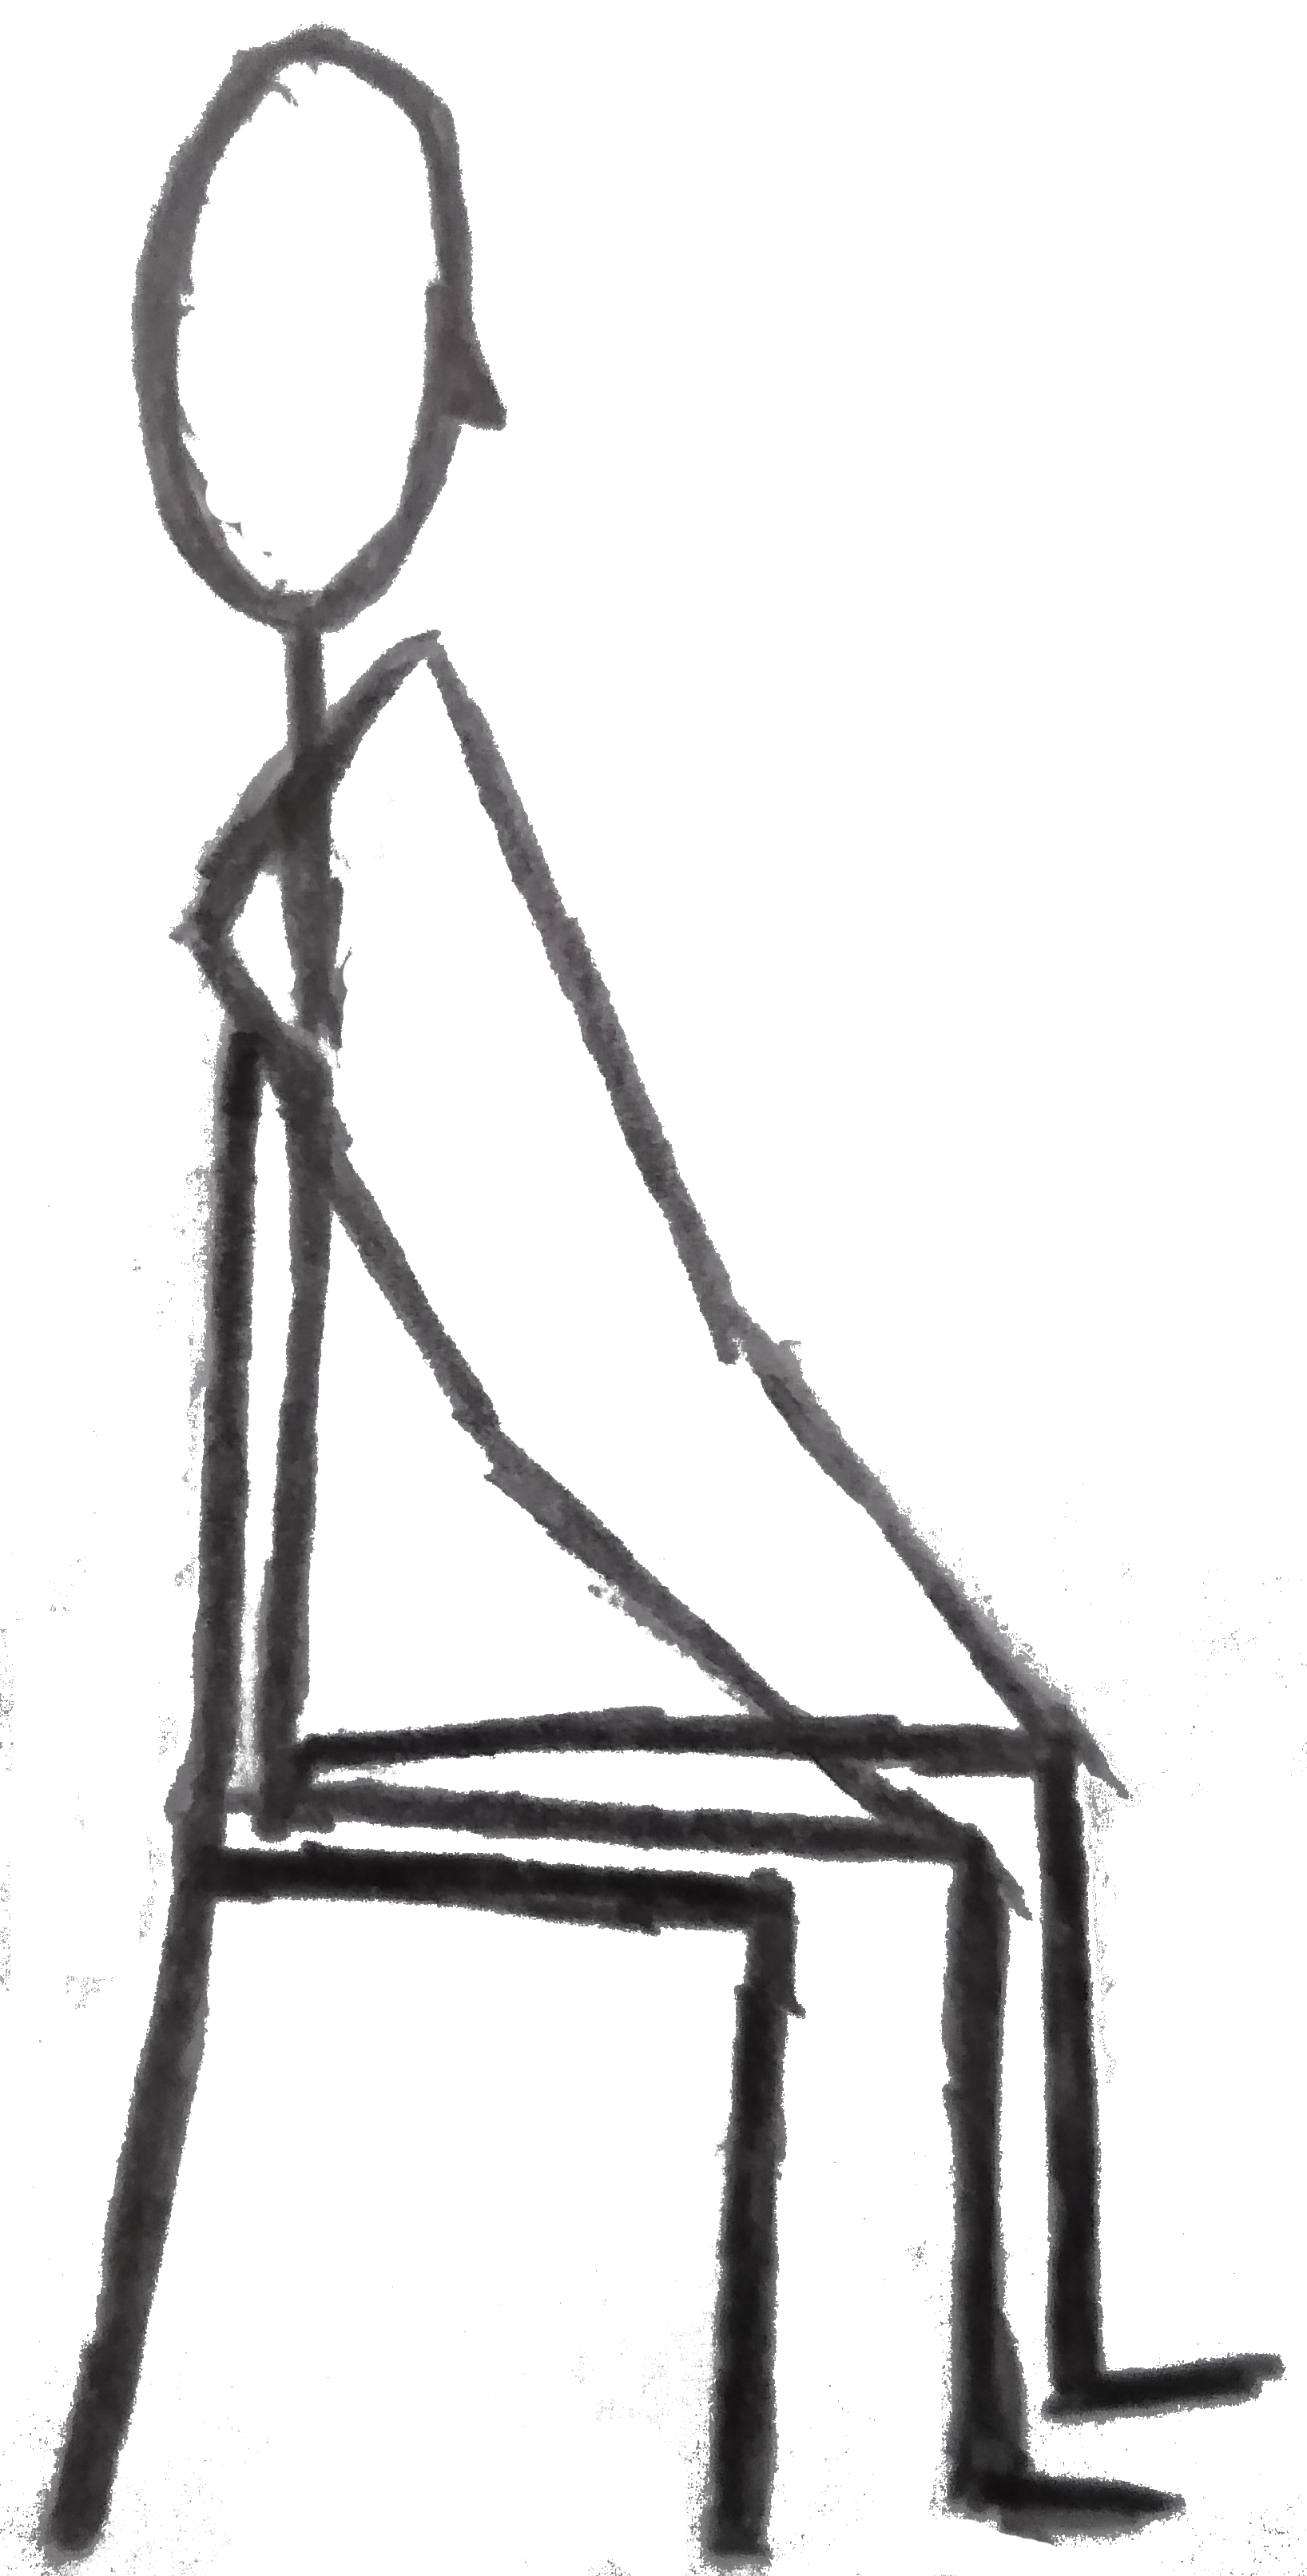
\includegraphics[width=\linewidth]{Sitting_chair_side.png}
\column{.7\textwidth} % Right column and width
In the center of the formal practice is the sitting meditation. In the \structure{sitting meditation}, we \structure{sit and breathe}: two activities we encounter everywhere in daily life. 

The sitting of the sitting meditation differs from the usual, daily sitting by the presence of our \structure{inner mindful attitude}. 
In the sitting meditation it is important to sit in a \structure{dignified posture}, with erect head, neck and back, without tensing up. 
You can use a chair with \structure{straight back rest} or on a pillow on the \structure{floor with your legs crossed}. 

The position should radiate and \structure{awake and dignified posture}.
\end{columns}
\end{frame}
%------------------------------------------------------------

\begin{frame}
\frametitle{Focus Point}
\begin{columns}[c] % The "c" option specifies centered vertical alignment while the "t" option is used for top vertical alignment

\column{.3\textwidth} % Left column and width
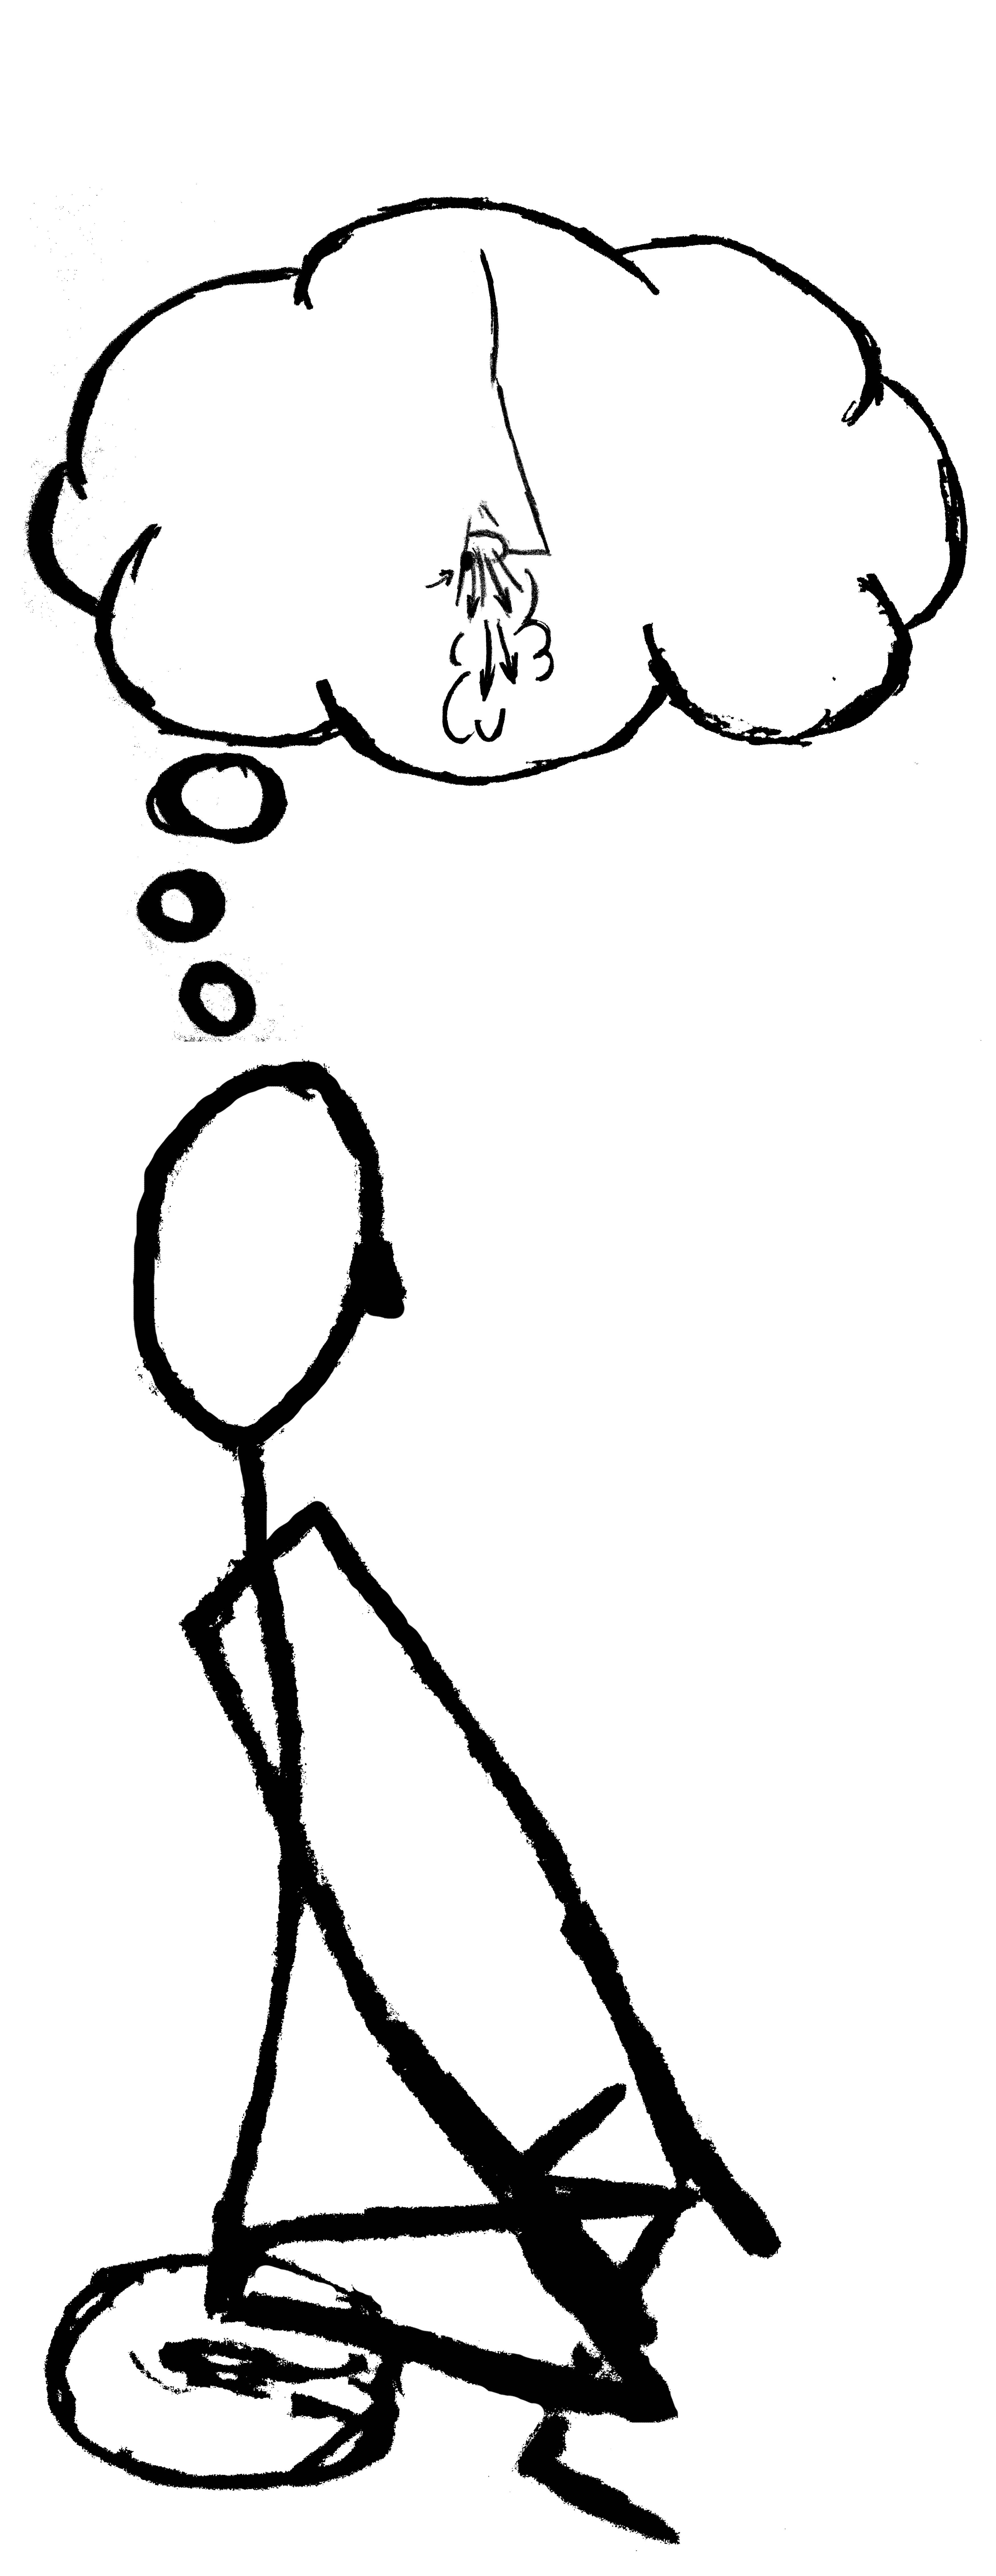
\includegraphics[width=\linewidth]{Thinking_man_breath.png}
\column{.65\textwidth} % Right column and width
Normally you start by choosing an \structure{object to focus the attention} - for instance your \structure{breath}. 

To be more precise, you focus on a single aspect of your breath, like the sensation of the \structure{air streaming in and out} at the back end of your nostrils or the gentle \structure{stretching and lowering of your abdominal wall} with each inhale and exhale. 
\end{columns}
\end{frame}
%------------------------------------------------------------

\begin{frame}
\frametitle{Widening your Focus}
\begin{columns}[c] % The "c" option specifies centered vertical alignment while the "t" option is used for top vertical alignment

\column{.3\textwidth} % Left column and width
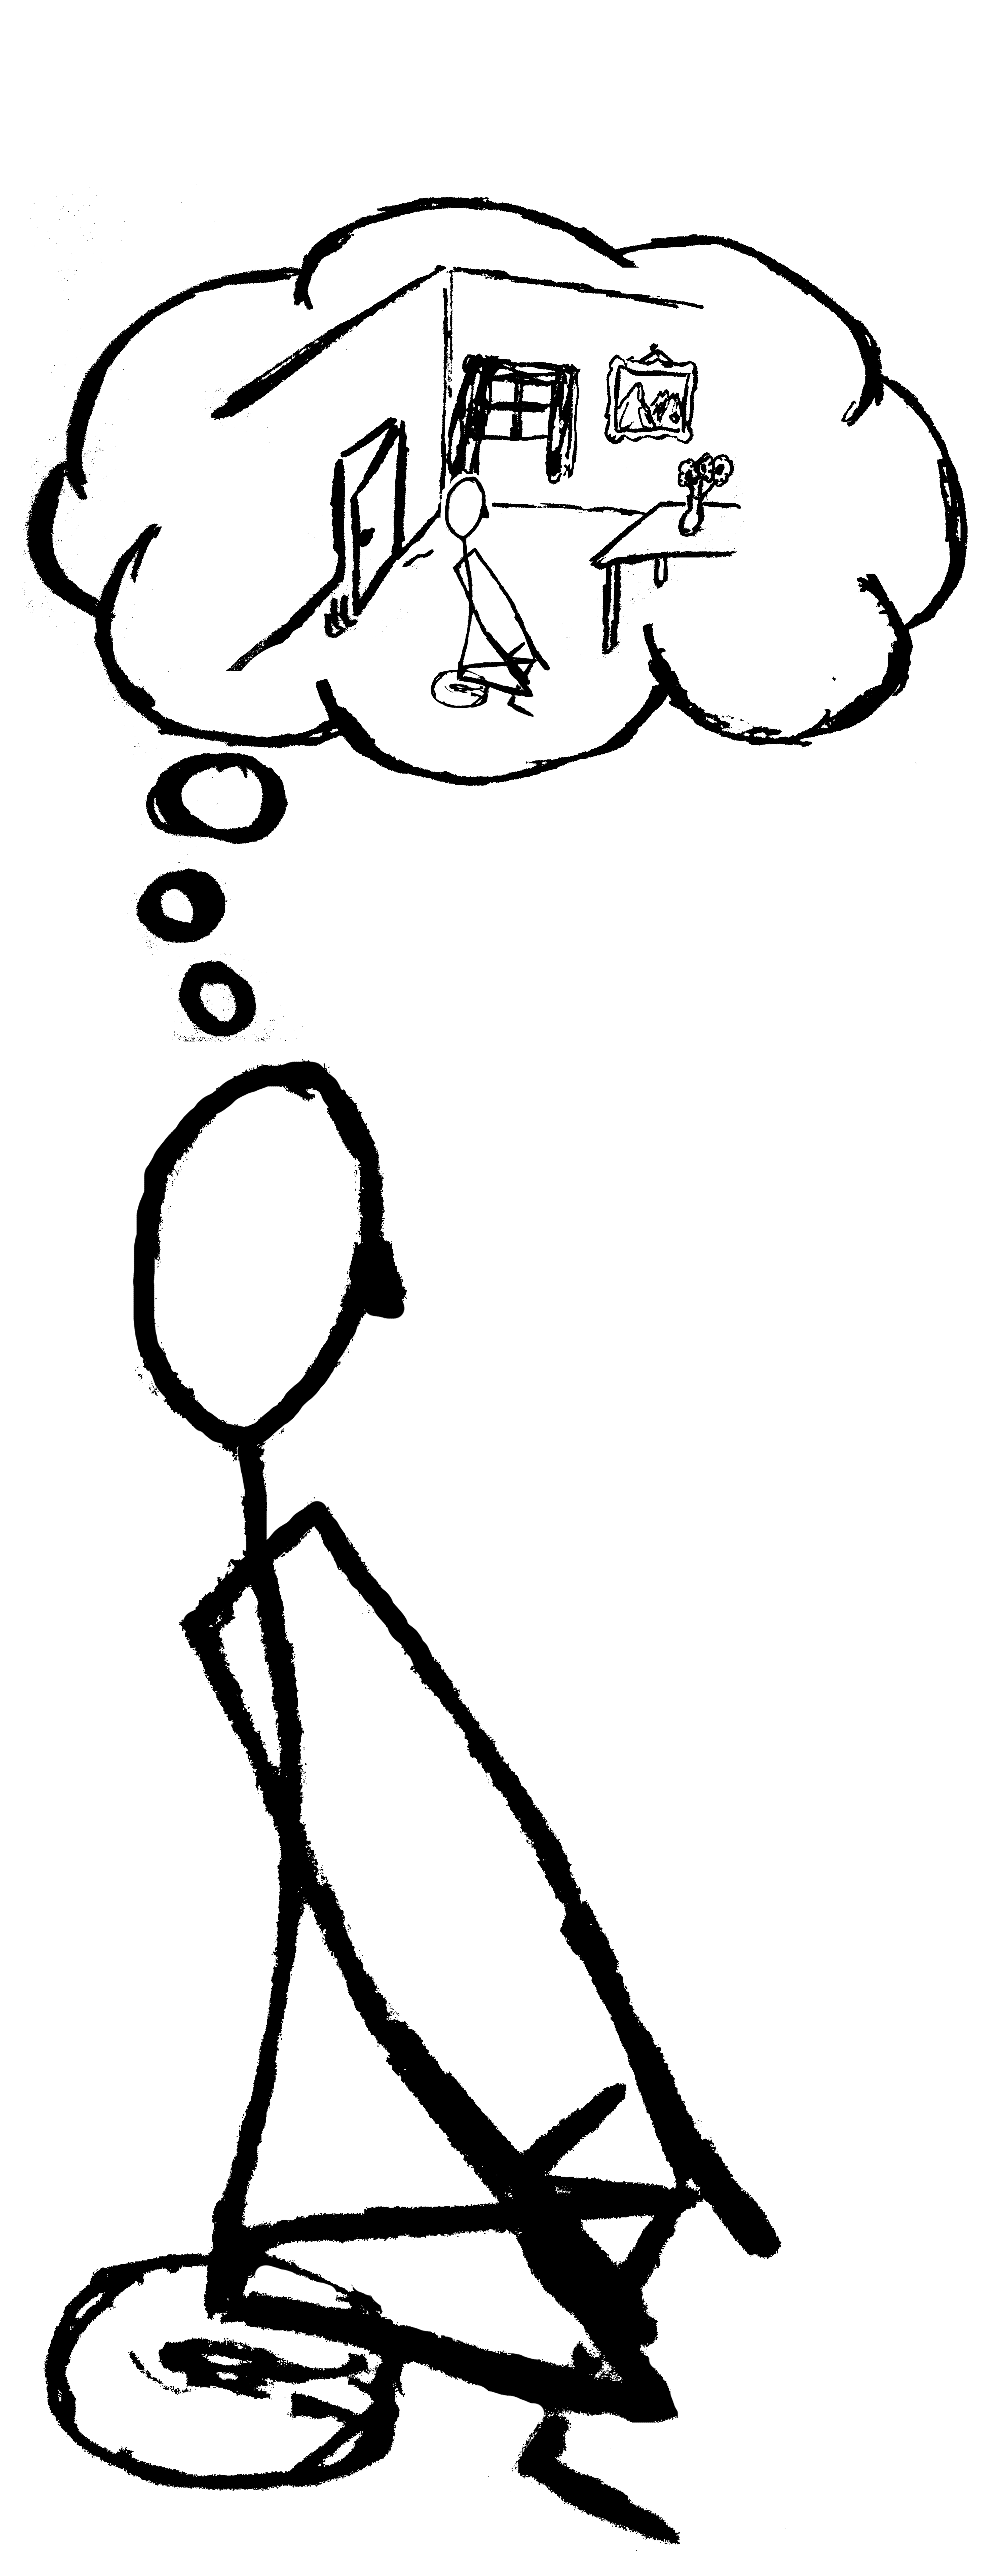
\includegraphics[width=\linewidth]{Thinking_man_thinkHouse.png}
\column{.65\textwidth} % Right column and width
Once a certain degree of focus developed, the \structure{attention can get widened} beyond the changing sensations of your breath. 

Sounds, perceptions, thoughts or other objects will be perceived in a heedful manner as soon as they enter your awareness. We try as good as possible to maintain a \structure{calm, non--reactive and steady awareness}, anchored by the breath.
\end{columns}

\end{frame}
%------------------------------------------------------------

\begin{frame}
\frametitle{What do you need for a sitting meditation?}

\begin{columns}[c] % The "c" option specifies centered vertical alignment while the "t" option is used for top vertical alignment

\column{.3\textwidth} % Left column and width
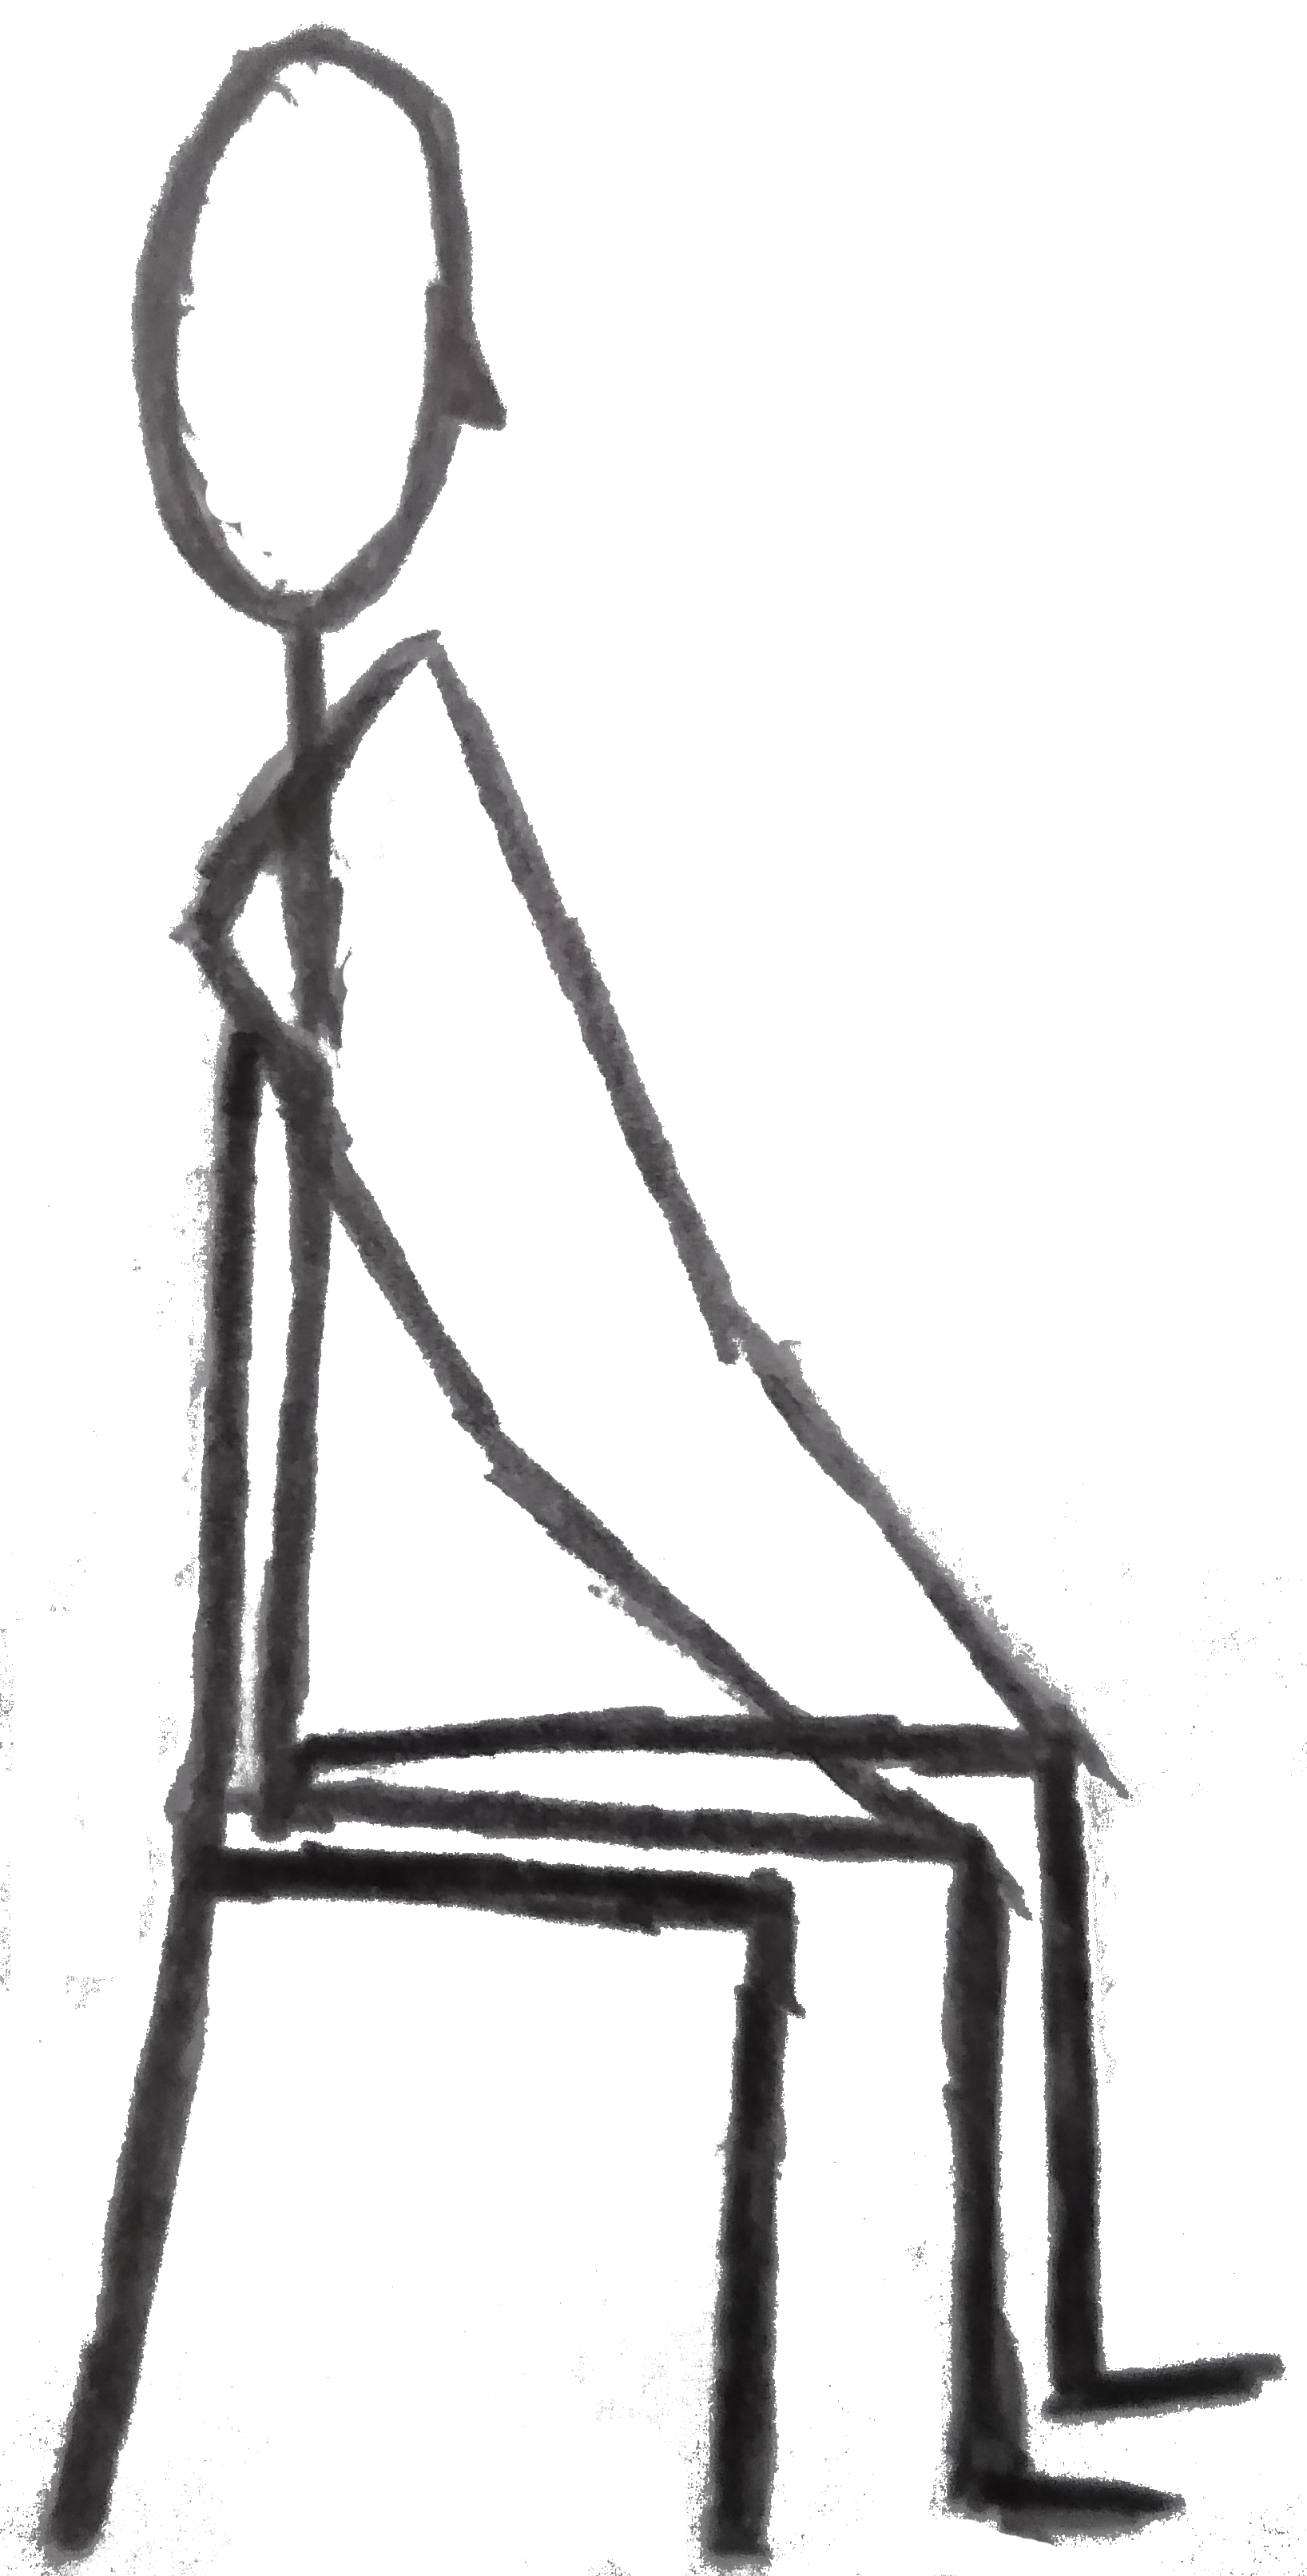
\includegraphics[width=\linewidth]{Sitting_chair_side.png}
\column{.7\textwidth} % Right column and width
\begin{itemize}
\item A \structure{fixed point of time}. 
\item A place where you can relatively \structure{undisturbed}. 
\item An \structure{upright posture} which allows you to sit for a prolonged period of time. 
\end{itemize}
Find a seat on a chair with straight back rest or on the floor. If you sit on a chair, both \structure{feet} should rest with the whole \structure{soles on the floor}. Most of the time it’s indicated to not use the back rest, but to keep your \structure{back free, straight and upright}. If this is too exhausting, then it’s preferable to lean against the backrest then to be constantly distracted by the unfamiliar strain.
\end{columns}
\end{frame}
%------------------------------------------------------------

\begin{frame}
\frametitle{Sitting on the floor}

\begin{columns}[c] % The "c" option specifies centered vertical alignment while the "t" option is used for top vertical alignment

\column{.3\textwidth} % Left column and width
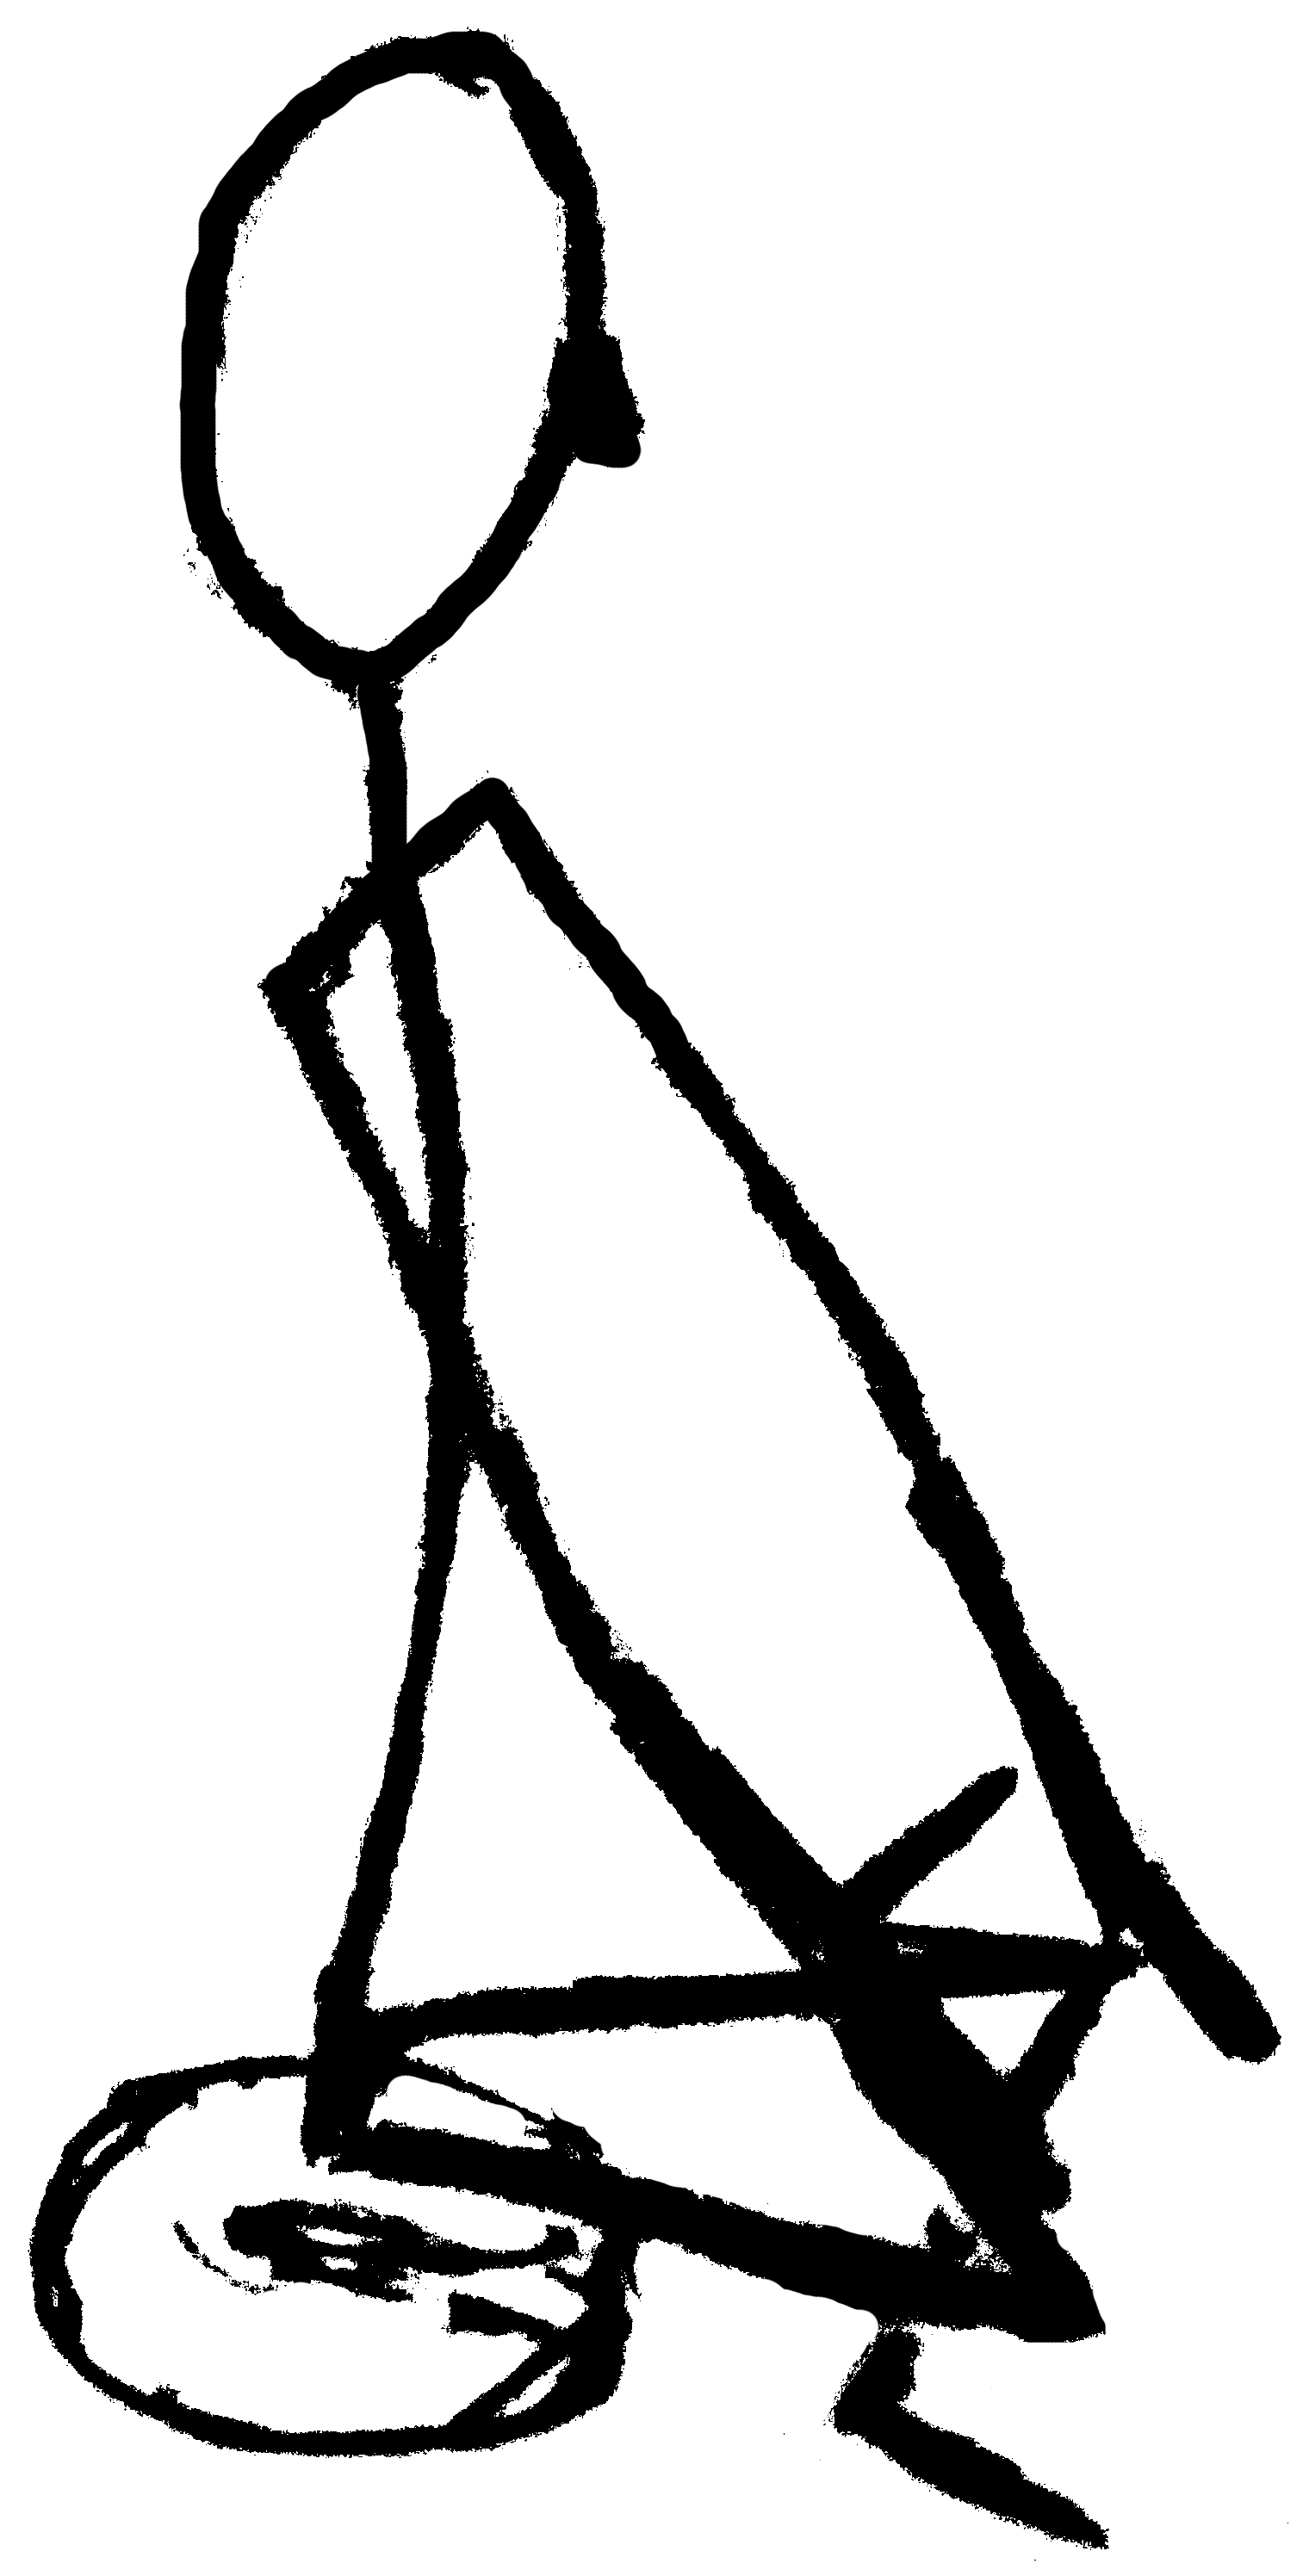
\includegraphics[width=\linewidth]{Sitting_floor_side.png}
\column{.6\textwidth} % Right column and width
When you sit on the floor, you can use a \structure{pillow to lift the buttocks} off the floor (that helps to keep the back straight). Take a \structure{regular pillow} which you \structure{fold} once or twice or then a special meditation pillow in wedge shape, a so called Zafu. The position sitting on the floor can give you the calming feeling of being \structure{stable and grounded}. 
\end{columns}
\end{frame}
%------------------------------------------------------------

\begin{frame}
\frametitle{Posture}
\begin{columns}[c] % The "c" option specifies centered vertical alignment while the "t" option is used for top vertical alignment

\column{.48\textwidth} % Left column and width
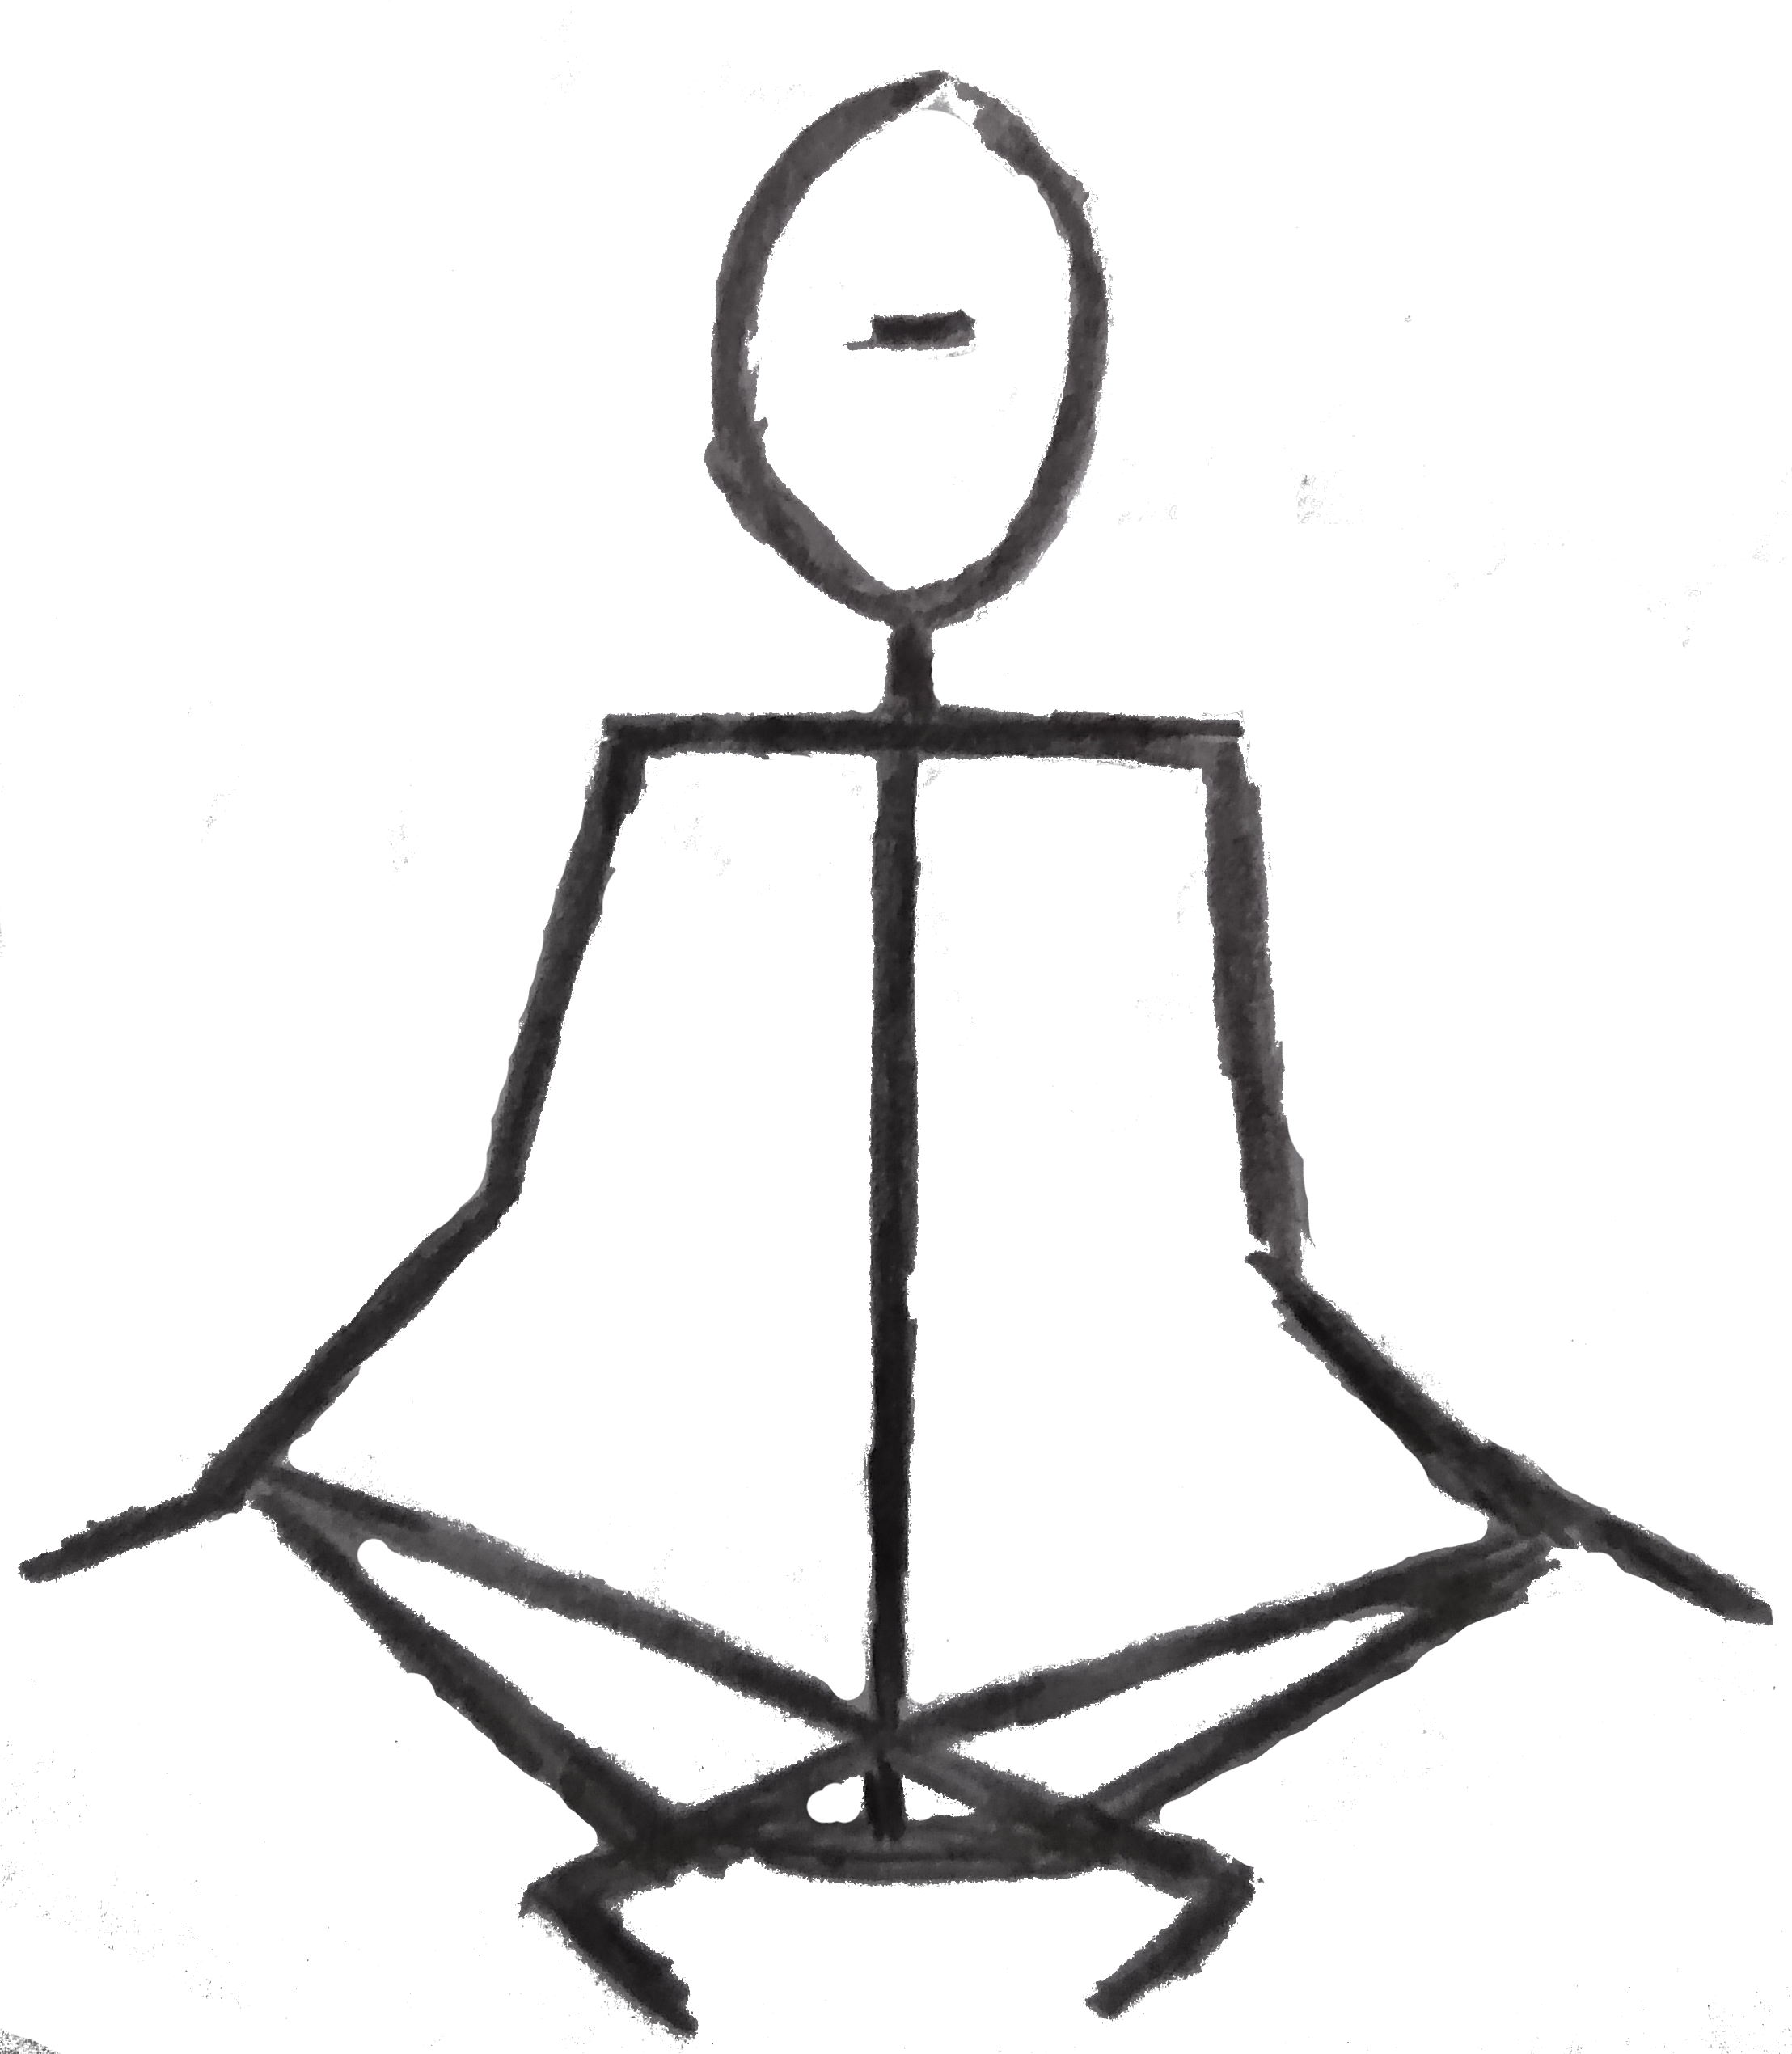
\includegraphics[width=\linewidth]{Sitting_floor_front.png}
\column{.55\textwidth} % Right column and width
Sitting on the floor isn't a condition for meditation, what really counts is the \structure{sincerity of your efforts}, not the surface you're sitting on. It's recommendable that the \structure{head, neck and back lie in a straight line} in order for the breath to flow effortlessly. This posture radiates a certain dignity and can progressively be an \structure{expression of the inner attitude, your self esteem, self--acceptance and the focussed attention} which you are cultivating. 
\end{columns}
\end{frame}
%------------------------------------------------------------

%------------------------------------------------------------

\begin{frame}
\frametitle{Follow your breath}
\begin{columns}[c] % The "c" option specifies centered vertical alignment while the "t" option is used for top vertical alignment

\column{.3\textwidth} % Left column and width
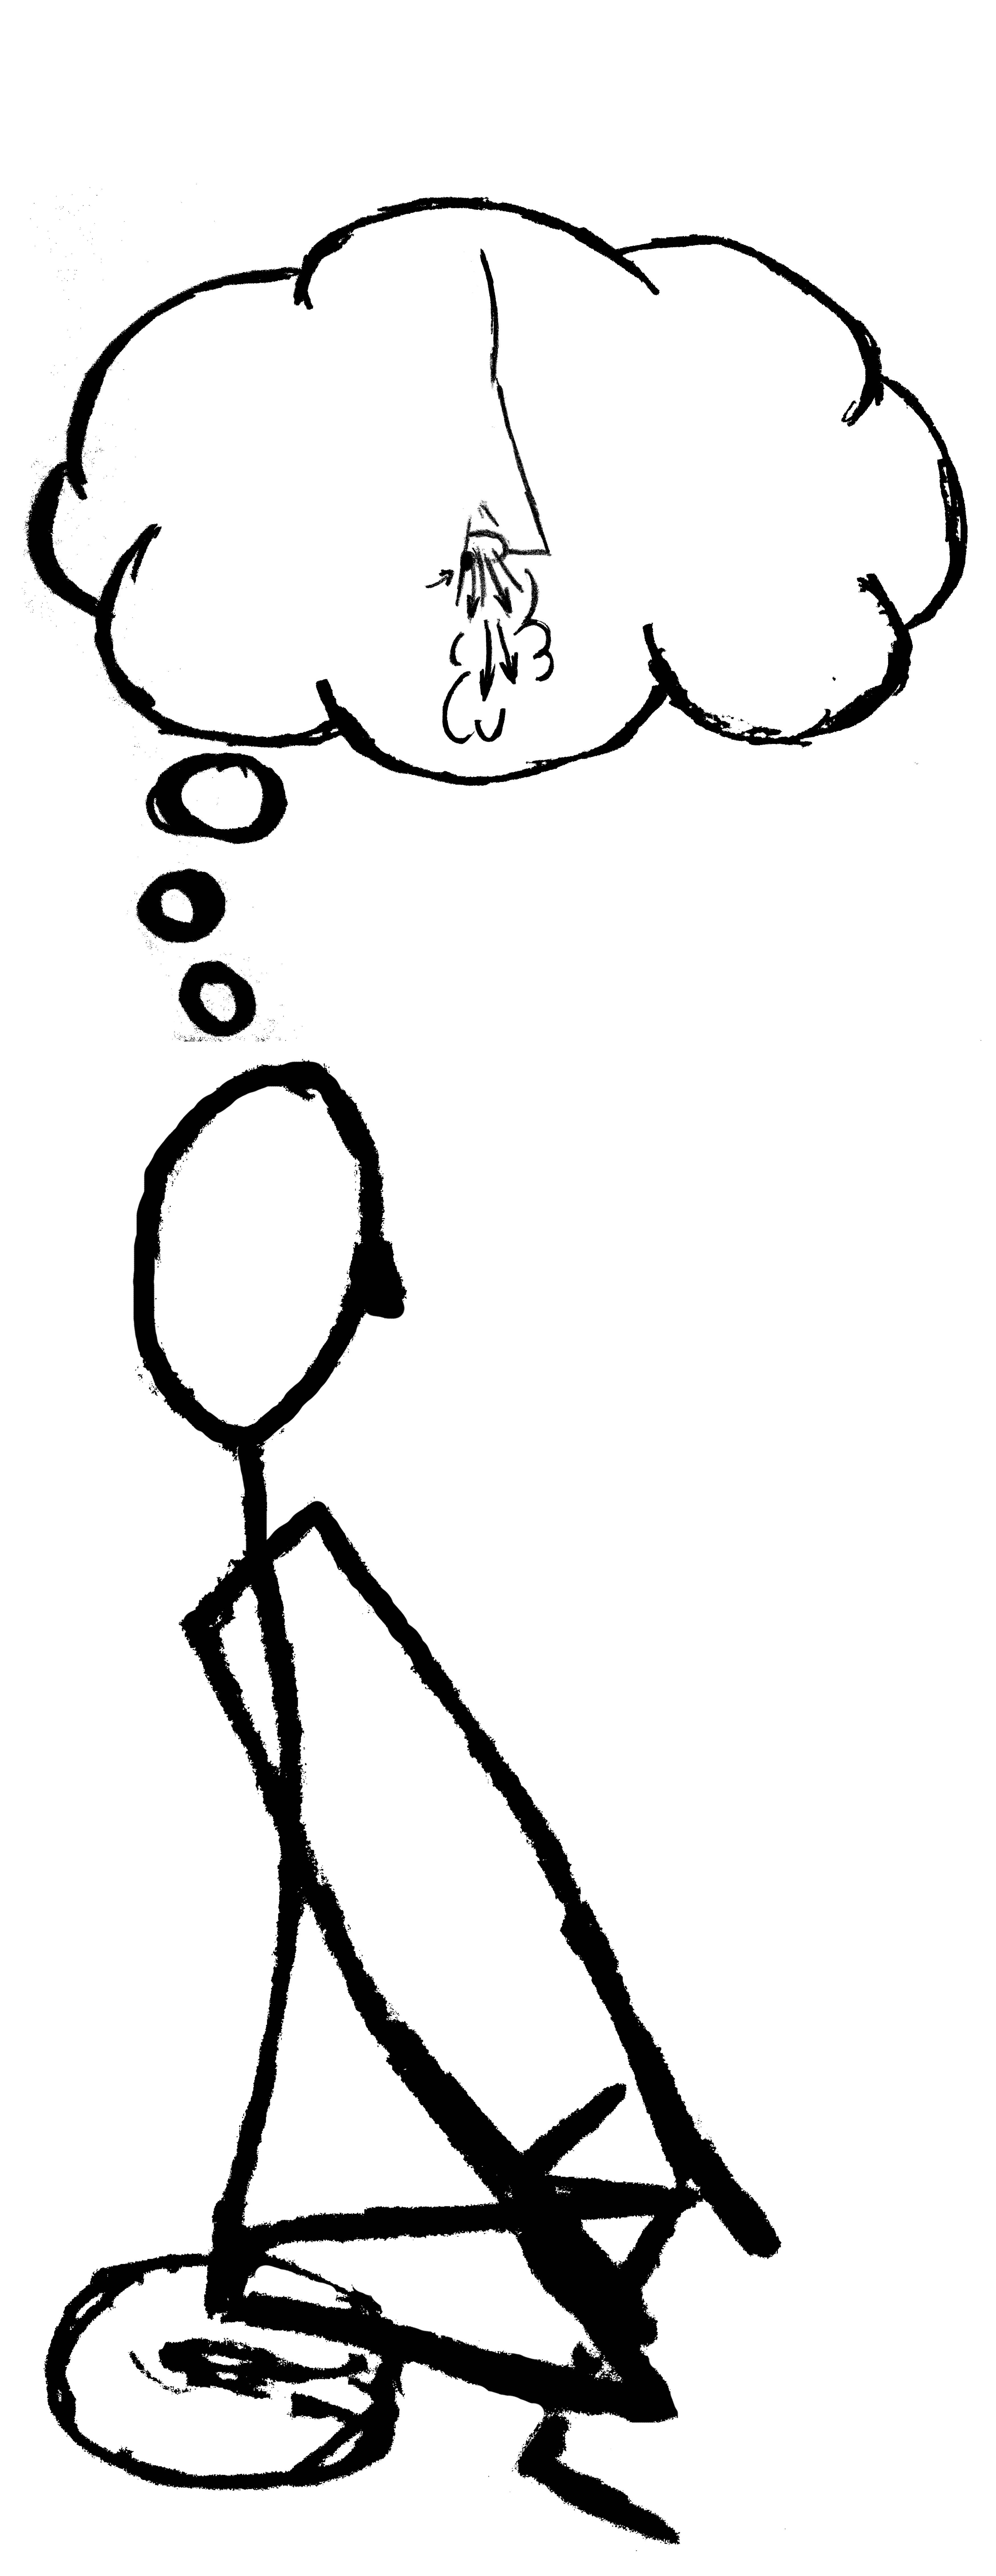
\includegraphics[width=\linewidth]{Thinking_man_breath.png}
\column{.65\textwidth} % Right column and width
Did you settle down in a position? Put your attention on the \structure{process of your breathing}. Feel consciously how the breath streams in and out. Let your breaths happen in a natural way and limit yourself to \structure{observe it} and to \structure{perceive all the related feelings}. Just take your sweet time and give your full attention to the inhale and the exhale. 
\end{columns}
\end{frame}
%------------------------------------------------------------

%------------------------------------------------------------

\begin{frame}
\frametitle{Distractions}
\begin{columns}[c] % The "c" option specifies centered vertical alignment while the "t" option is used for top vertical alignment

\column{.3\textwidth} % Left column and width
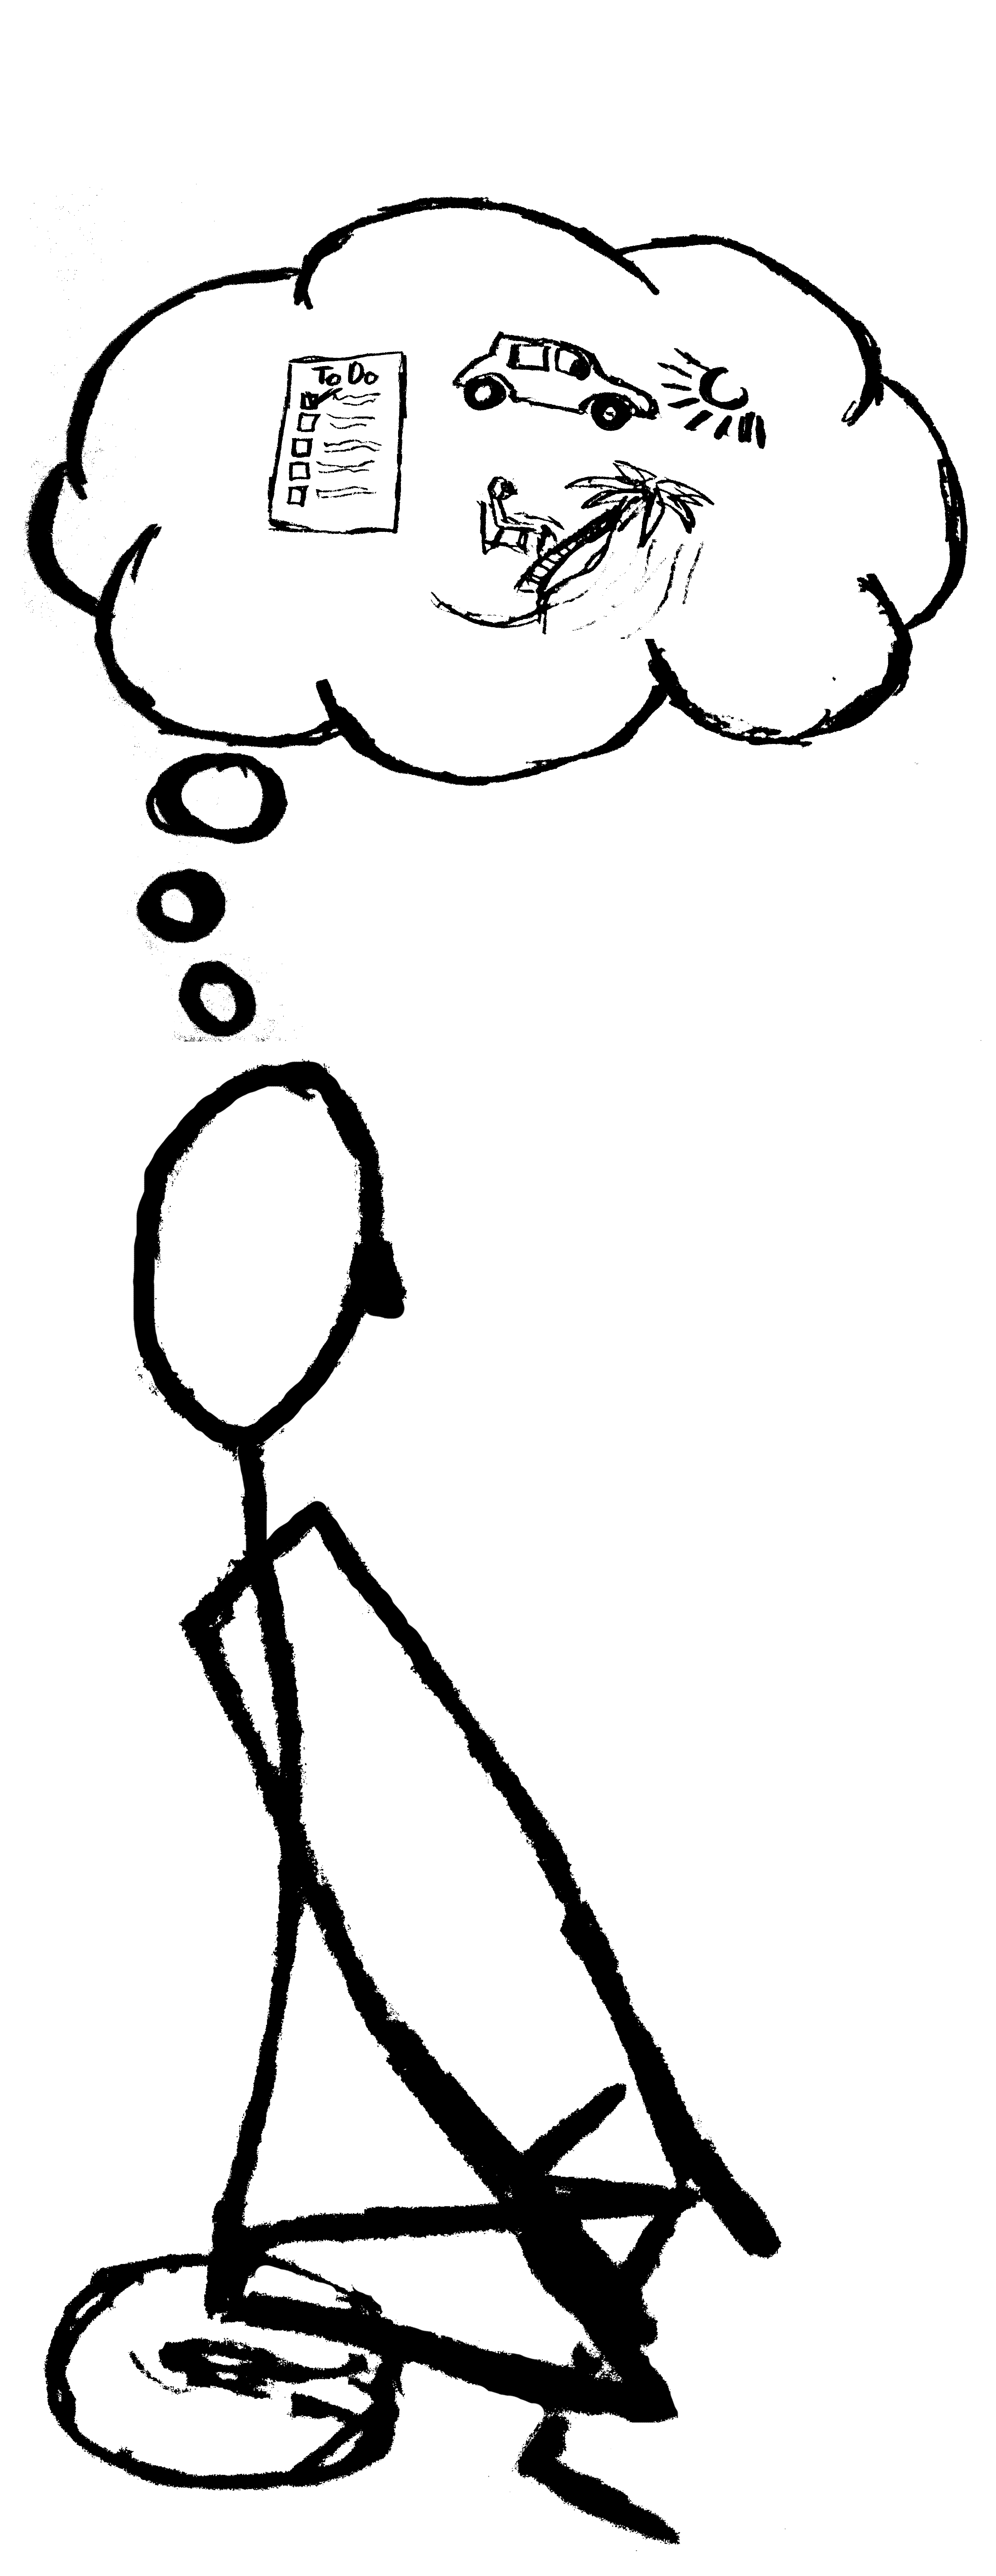
\includegraphics[width=\linewidth]{Thinking_man.png}
\column{.65\textwidth} % Right column and width
Perhaps your body will urge you to to change the position, perhaps your \structure{thoughts wander} to other topics.
That is totally \structure{normal and unavoidable}. In this case you can try to bring your attention back to your respiration gently but in a determined way. Don't let yourself \structure{being distracted by your wandering thoughts} or by your restless body: \structure{Stay patient} and don't get angry.
\end{columns}
\end{frame}
%------------------------------------------------------------
%------------------------------------------------------------

\begin{frame}
\frametitle{Your thoughts have their own will}
\begin{columns}[c] % The "c" option specifies centered vertical alignment while the "t" option is used for top vertical alignment

\column{.3\textwidth} % Left column and width
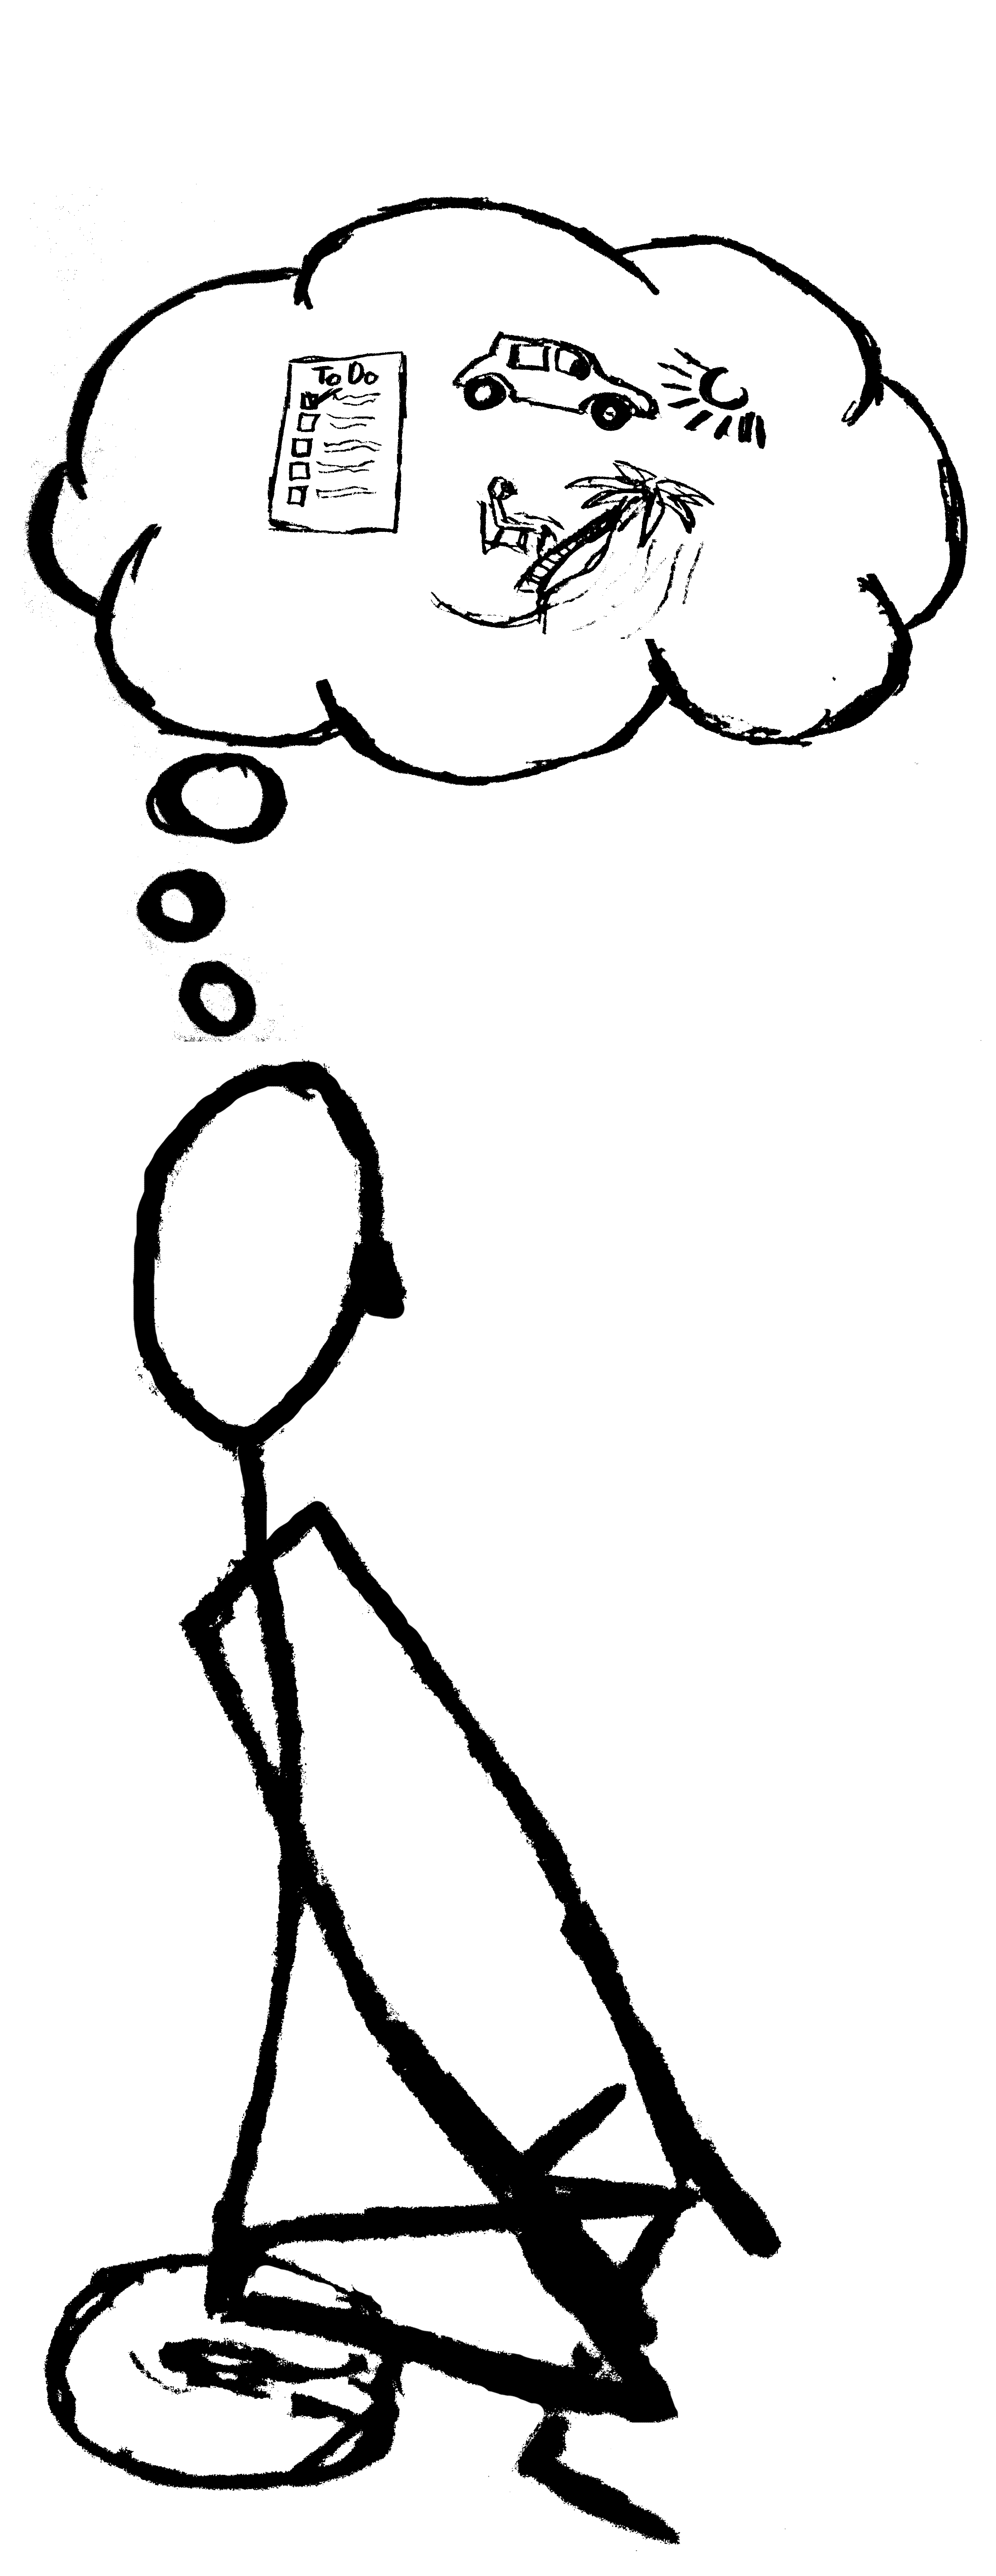
\includegraphics[width=\linewidth]{Thinking_man.png}
\column{.65\textwidth} % Right column and width
\begin{itemize}
\item[-]You will probably notice, that your \structure{thoughts follow their own trajectories}: Even though you were seriously committed to follow your breath, your \structure{thoughts wandered} to other topics; the conscious monitoring of your breath is forgotten. 
\item[-]Instead of getting upset, just try to continuously \structure{lead your thoughts back to your breath}, without complaining about the digression. 
\end{itemize}
\end{columns}
\end{frame}
%------------------------------------------------------------
%------------------------------------------------------------

\begin{frame}
\frametitle{Your thoughts}
\begin{columns}[c] % The "c" option specifies centered vertical alignment while the "t" option is used for top vertical alignment

\column{.3\textwidth} % Left column and width
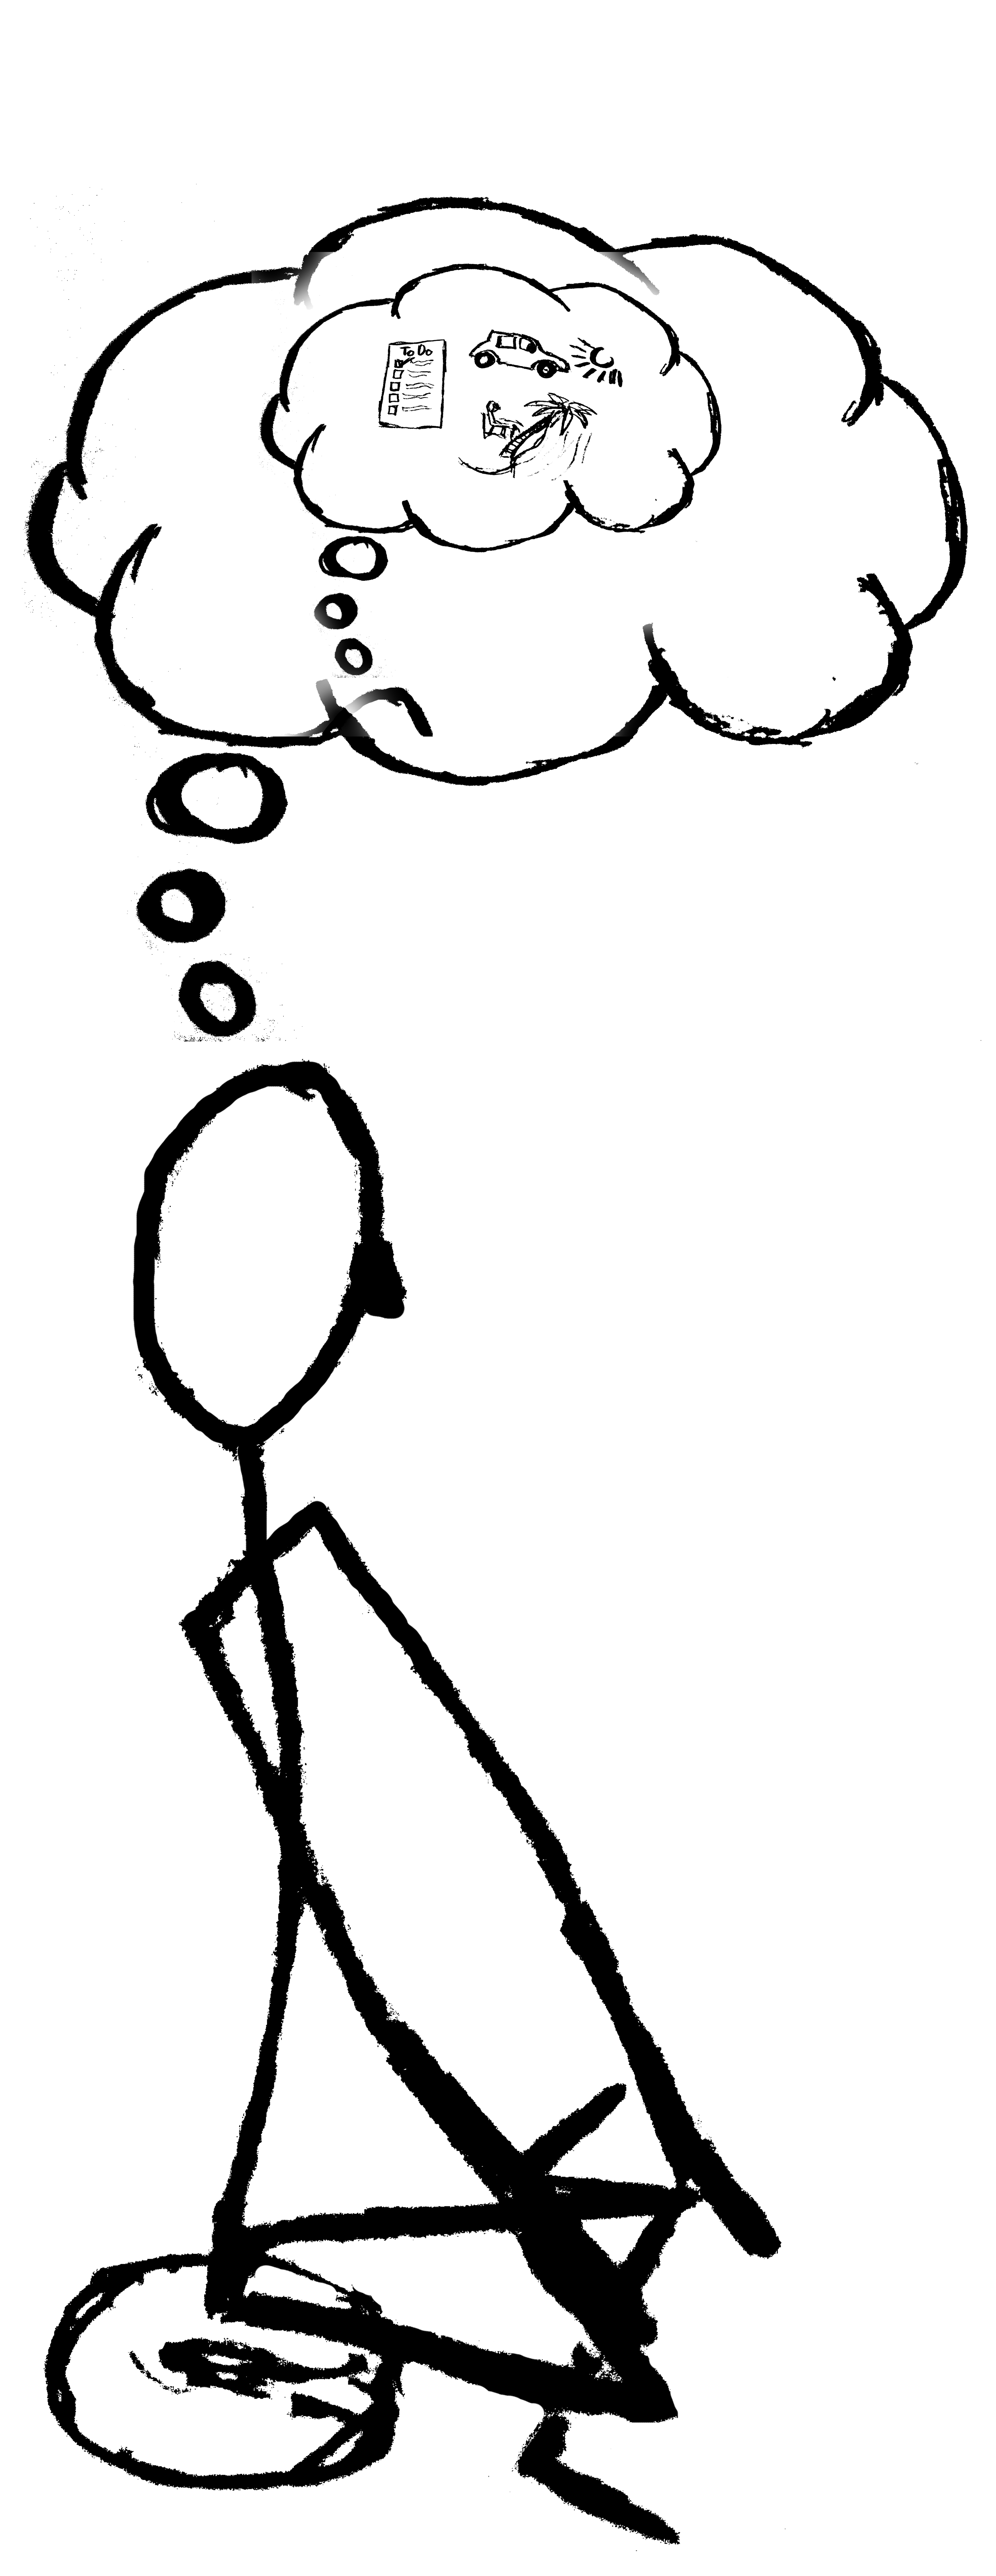
\includegraphics[width=\linewidth]{Thinking_man_thoughts.png}
\column{.65\textwidth} % Right column and width

\begin{itemize}
\item[-]Your thoughts are neither good nor bad. In meditation it only counts if you’re \structure{aware of your thoughts and how you deal with them}.
\item[-]Don't try to suppress your thoughts: just \structure{register their content and intensity} and let them \structure{wander} by. 
\item[-]Your thoughts are first and foremost \structure{impulses, which you can follow} -- or not. To recognize that can free us from the idea, that thoughts are uncontrollable realities.
\end{itemize}
\end{columns}
\end{frame}
%------------------------------------------------------------
%------------------------------------------------------------

\begin{frame}
\frametitle{Bodily distractions}
\begin{columns}[c] % The "c" option specifies centered vertical alignment while the "t" option is used for top vertical alignment

\column{.3\textwidth} % Left column and width
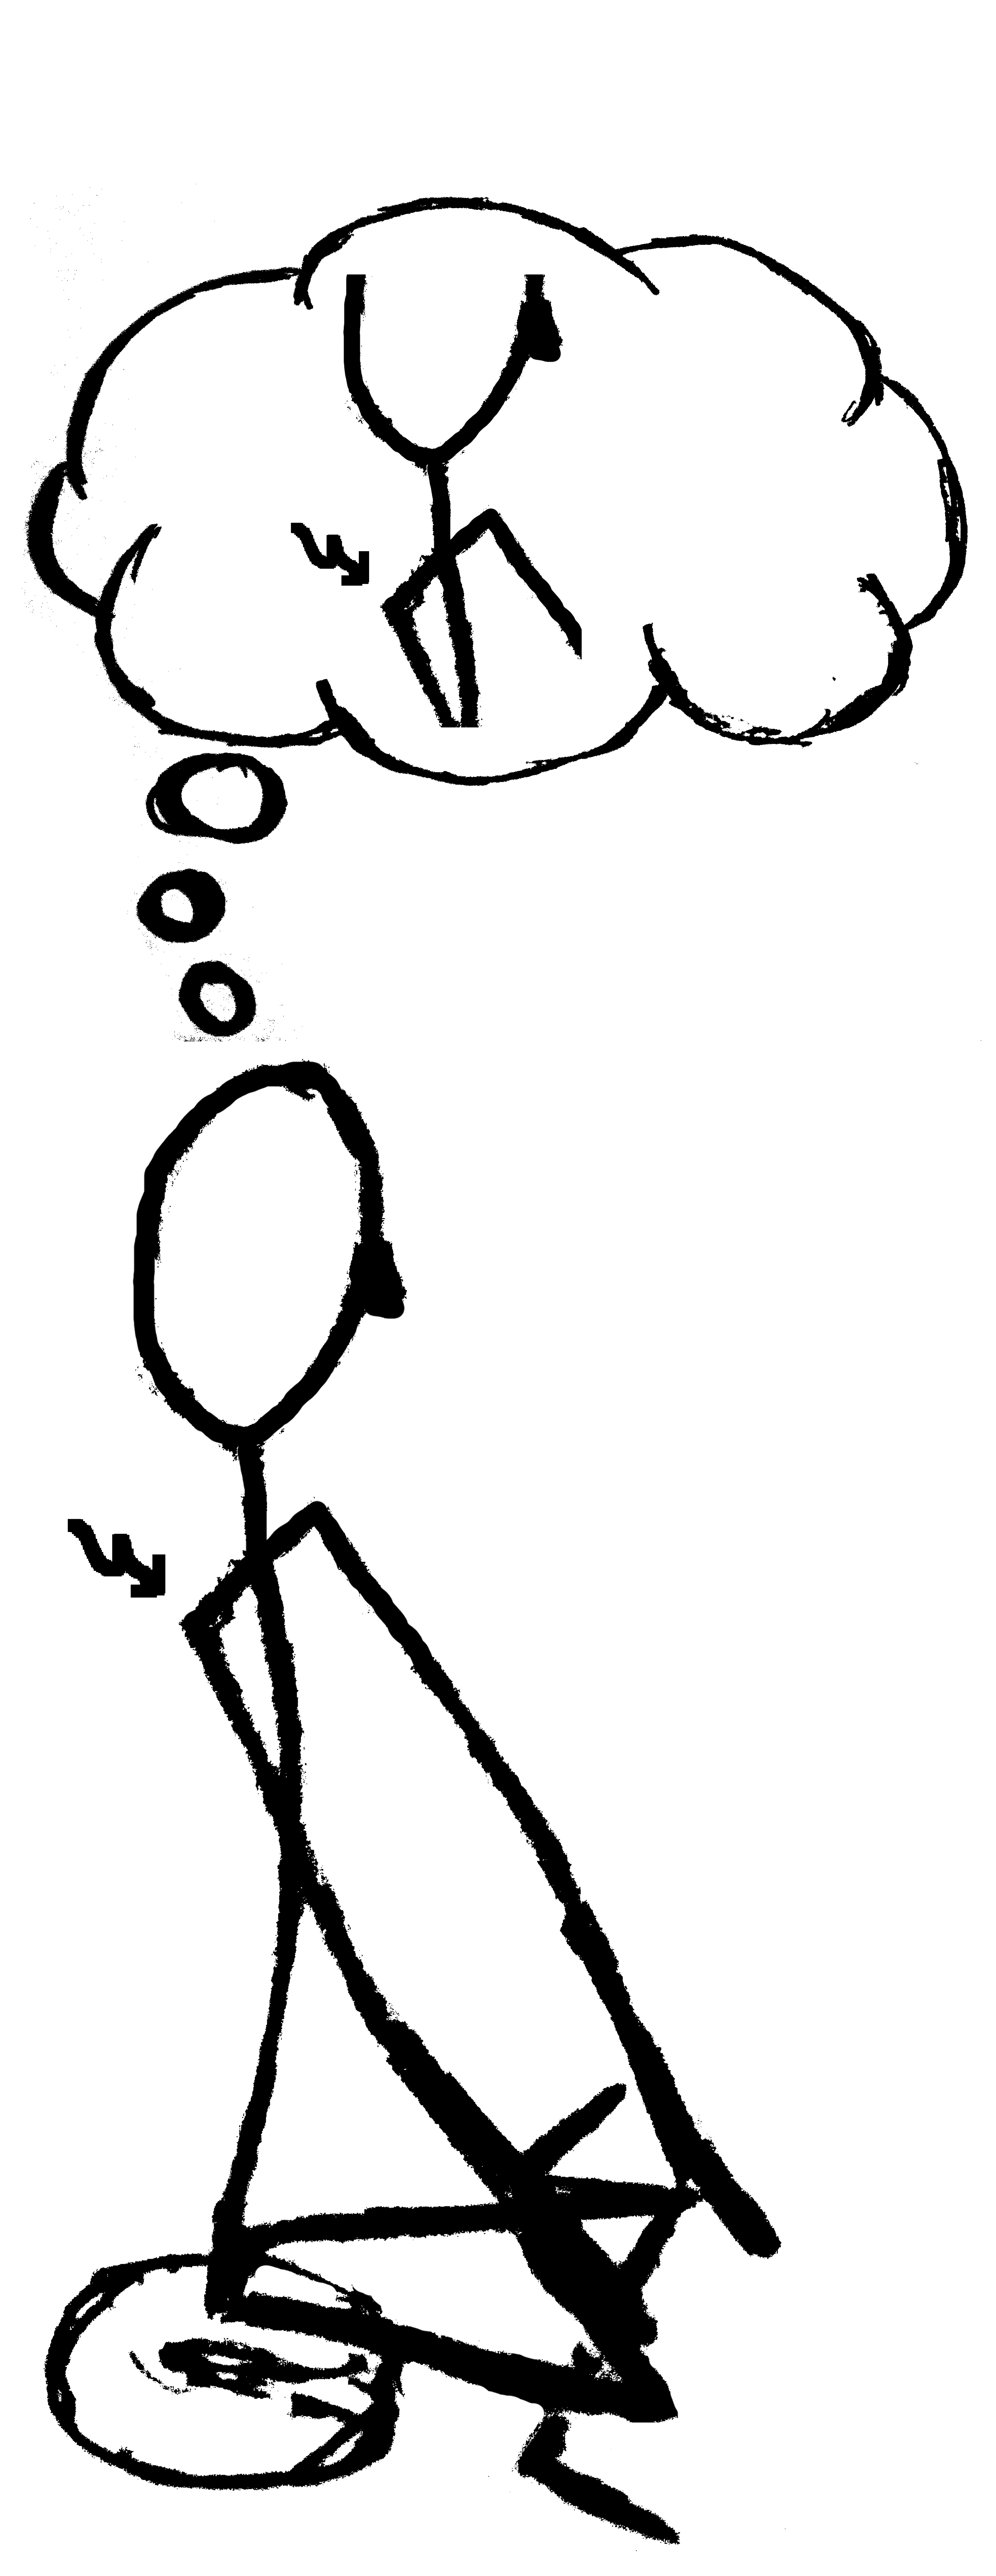
\includegraphics[width=\linewidth]{Thinking_man_body.png}
\column{.65\textwidth} % Right column and width

The strongest distractions will come from your body. Again and again will you feel impulses, like stretching your leg or shifting your weight. In meditation you should attempt to \structure{resist these impulses}. Take the \structure{unease you're feeling as a given}.

Even though the sensations of your body can indeed be \structure{uncomfortable}, you can still help them to unfold to \structure{calm, serenity and focus}. That's the only way to make the experience that \structure{you can relax regardless of physical afflictions}. In case there's no other way and you really have to change posture: please do this mindfully and focussed.
\end{columns}
\end{frame}
%------------------------------------------------------------










